\documentclass[tikz]{standalone}
\usepackage{pgfplots}
\pgfplotsset{compat=1.15}
\usepackage{mathrsfs}
\usetikzlibrary{arrows,calc}
\usepackage{tkz-euclide}

\pagestyle{empty}

\definecolor{AngleClr}{rgb}{0,0.39215686274509803,0}
\definecolor{ShapeClr}{rgb}{0.6,0.2,0}
\definecolor{ParacircleClr}{RGB}{217,185,7}

\begin{document}

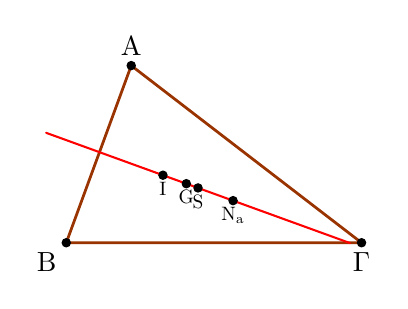
\begin{tikzpicture}[scale=.75]
\tkzSetUpLine[line width=1pt,color=black]
\tkzSetUpPoint[fill=black]

\tkzDefPoints{0/0/B,1.1/3/A,5/0/C}

\tkzDefMidPoint(B,C) \tkzGetPoint{MA}
\tkzDefMidPoint(A,C) \tkzGetPoint{MB}
\tkzDefMidPoint(A,B) \tkzGetPoint{MC}

\tkzInterLL(B,MB)(C,MC)\tkzGetPoint{G}
\tkzInCenter(A,B,C)\tkzGetPoint{I}
\tkzInCenter(MA,MB,MC)\tkzGetPoint{S}


\tkzDefTriangleCenter[nagel](A,B,C)\tkzGetPoint{Na}

\tkzFillPolygon[fill=white](A,B,C)
\tkzDrawPolygon[color=ShapeClr](A,B,C)

\tkzDrawSegment[line width=0.75pt, red, add=2.5 and 3.0](Na,G)
\tkzDrawPoints[size=3](I,G,S,Na)
\tkzDrawPoints[size=3](B,C,A)

\tkzLabelPoint[above](A){$\rm A$}
\tkzLabelPoint[below left](B){$\rm B$}
\tkzLabelPoint[below ](C){$\rm \Gamma$}
\tkzLabelPoint[below,scale=0.7](G){$\rm G$}
\tkzLabelPoint[below,scale=0.7](I){$\rm I$}
\tkzLabelPoint[below,scale=0.7](S){$\rm S$}
\tkzLabelPoint[below,scale=0.7](Na){$\rm N_a$}

\end{tikzpicture}

\end{document}
